% ==============================================================================
% SECTION 2: VALIDATION OF THE DATASET
% ==============================================================================
\section{Dataset Validation}

\begin{frame}{Dataset Validation}
    \begin{columns}[T]
        % --- Left Column: Filtering Criteria ---
        \begin{column}{0.54\textwidth}

            \begin{block}{Cleaning the data}
                \textbf{Remove lines that includes:}
                \begin{itemize}
                    \item Frozen sensor for 2+ seconds 
                    \item 5+ diverging values
                \end{itemize}
            \end{block}

            \begin{block}{Normalisation}
                \begin{itemize}
                    \item Directly in the training 
                \end{itemize}
            \end{block}

        \end{column}

        % --- Right Column: Visual Result / Impact ---
        \begin{column}{0.44\textwidth}
            
            \begin{block}{Static characteristic}
                \centering
                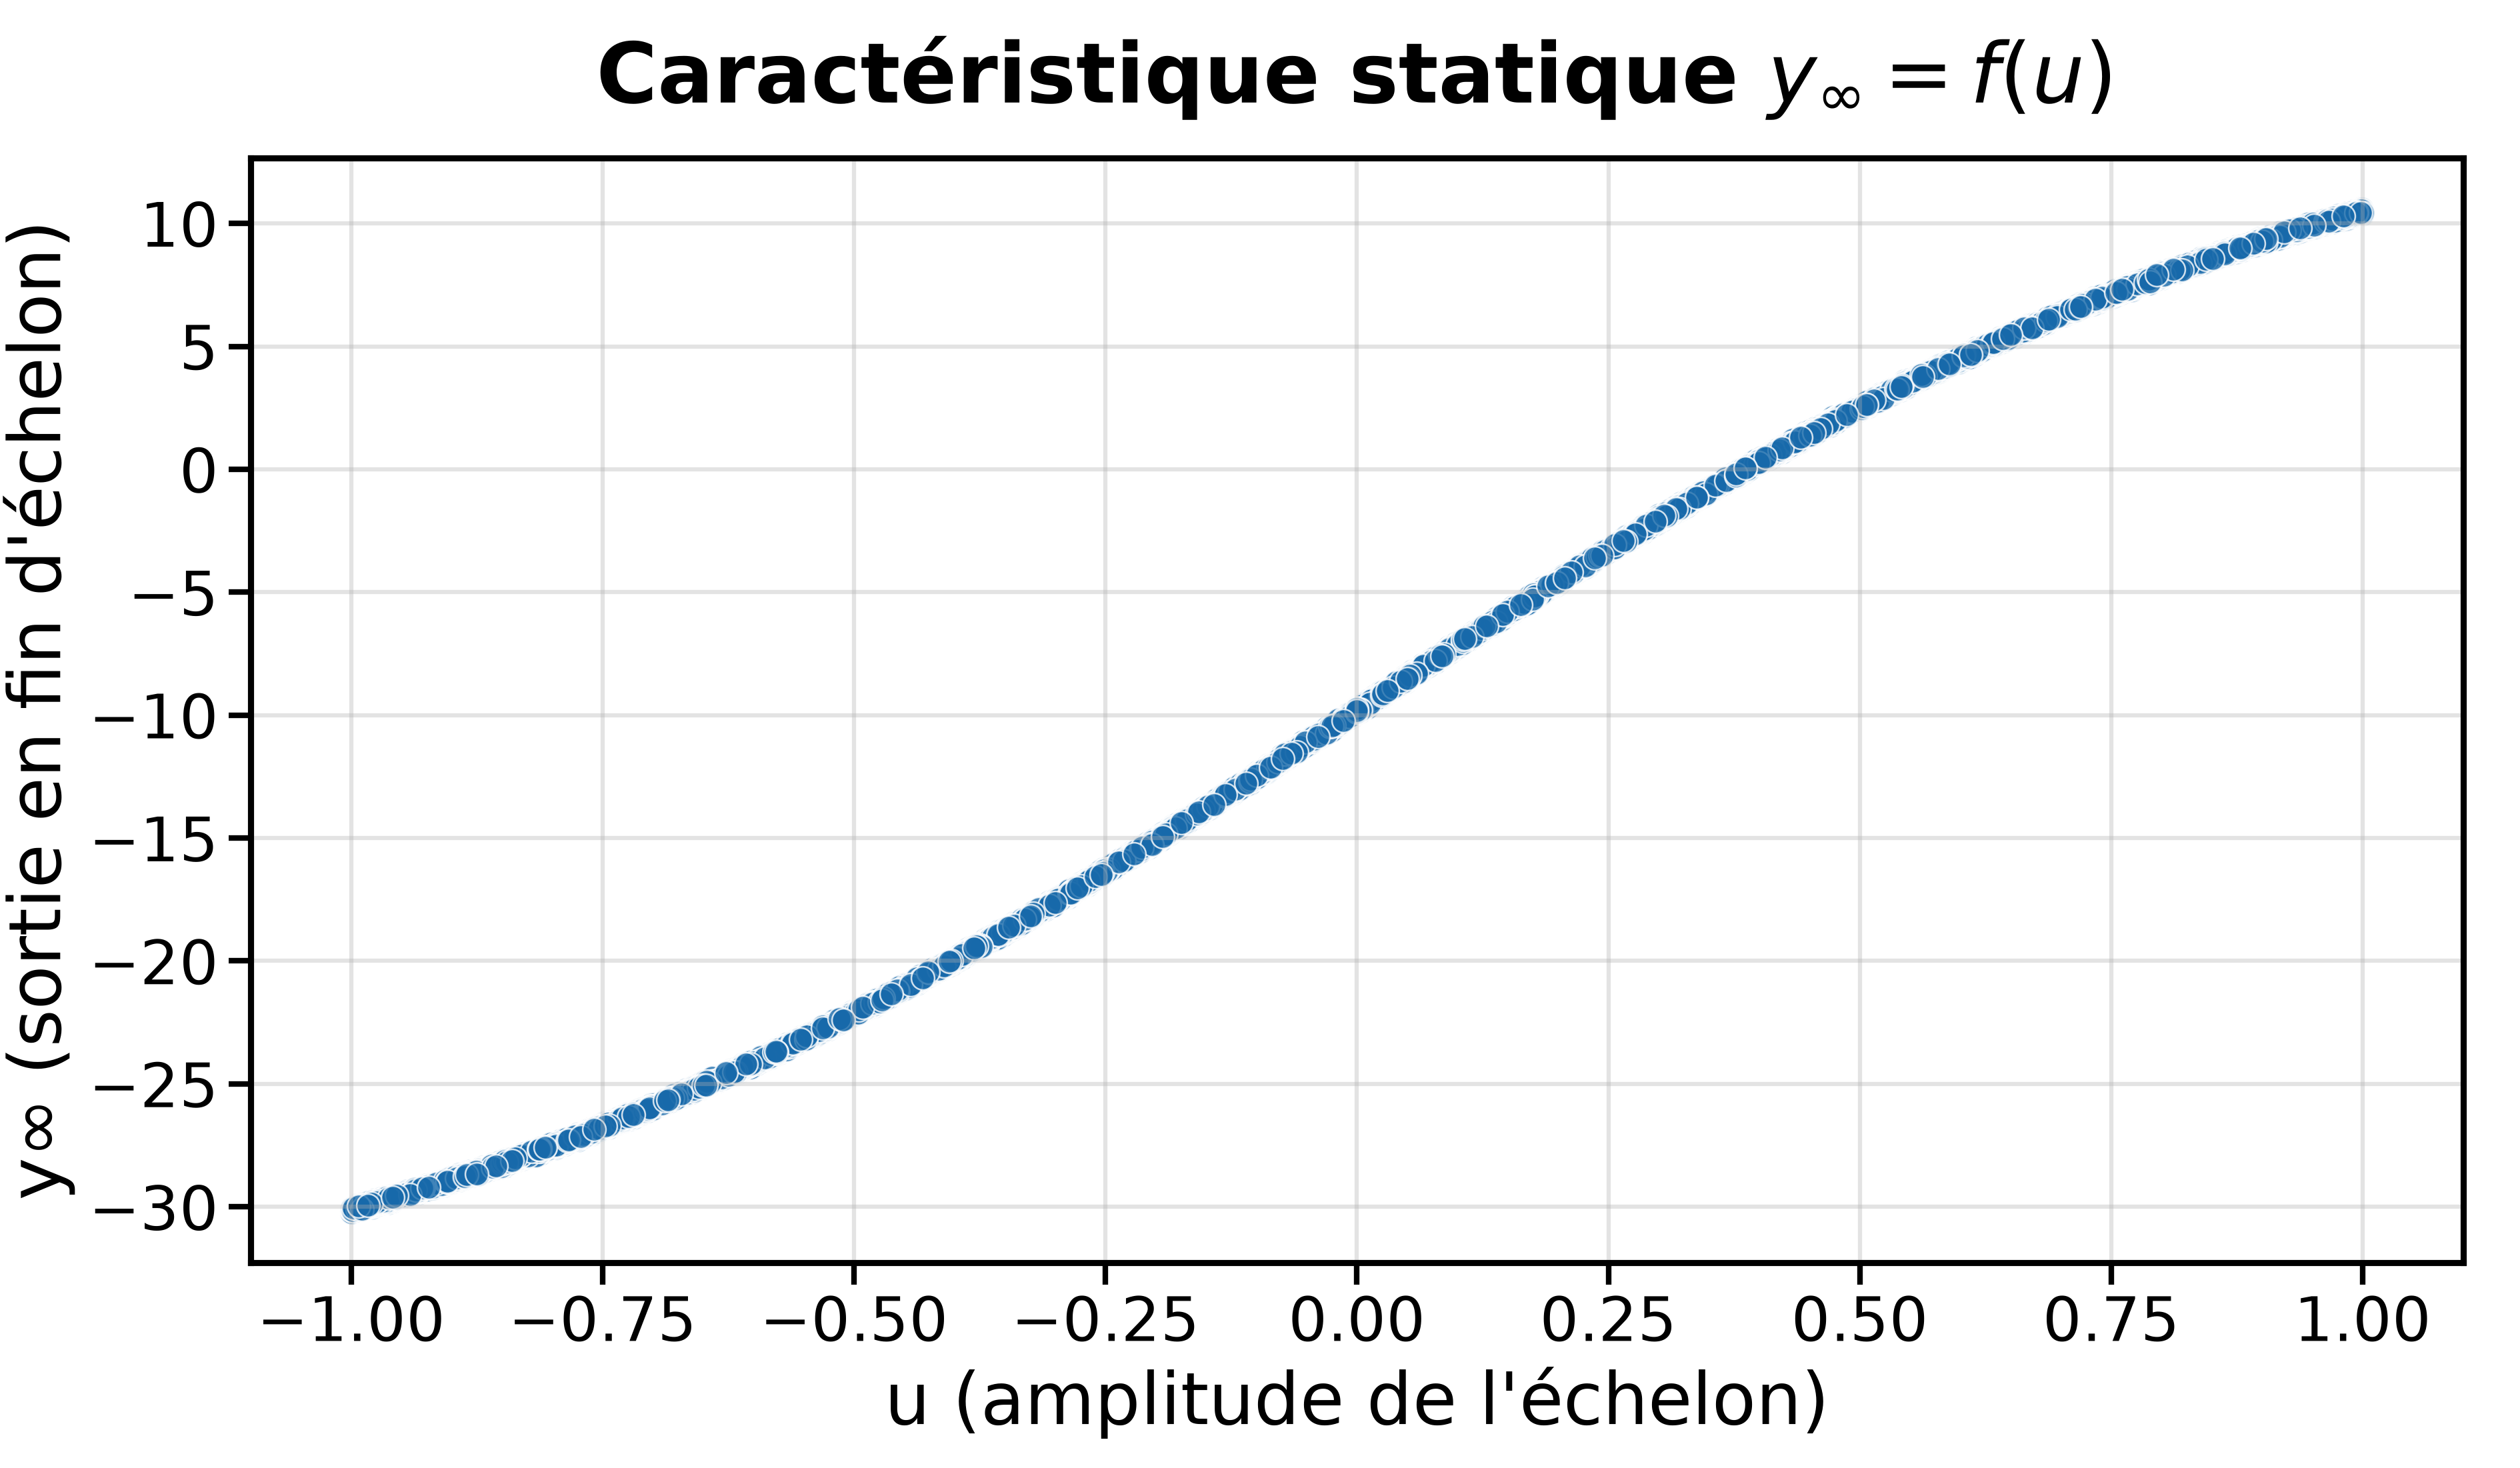
\includegraphics[
                    width=\linewidth,
                    height=5.0cm,
                    keepaspectratio
                ]{dataset_static_characteristic.png}
                % \vspace{0.1em}
                
                {\scriptsize $y_\infty = f(u)$ after eliminating corrupted runs.}
            \end{block}

        \end{column}
    \end{columns}
\end{frame}
